\begin{infocard}{La Hipotenusa}
    \begin{minipage}{0.36\textwidth}
        \begin{figure}[H]
            \centering
            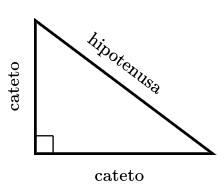
\includegraphics[width=0.99\linewidth]{../images/20230402132954.png}
        \end{figure}
    \end{minipage}\hfill
    \begin{minipage}{0.63\textwidth}
        La \textbf{hipotenusa} es el lado más largo y está enfrente del ángulo recto (ver Figura). Los dos catetos son los lados más cortos que forman el ángulo recto:
    \end{minipage}
\end{infocard}%